% !TEX root = main.tex

\section{简介} % ch1
\begin{figure}[!htbp]
\centering
\begin{tabular}{cc}
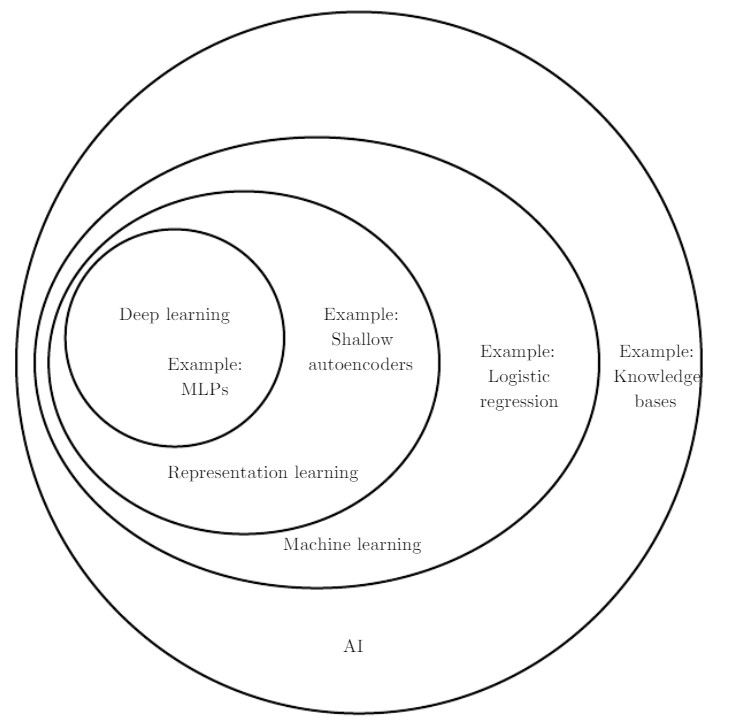
\includegraphics[width=0.5\linewidth]{fig/dl_venn.jpg}
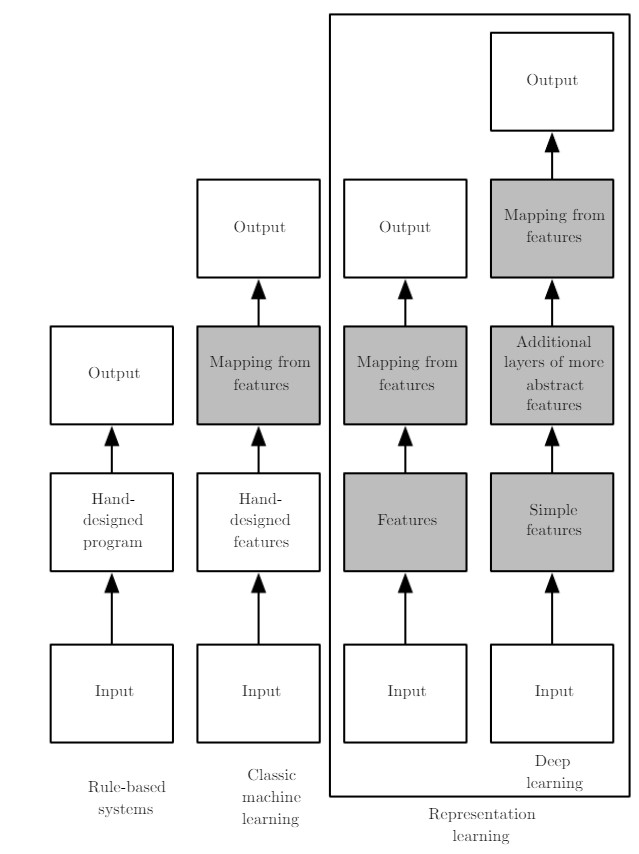
\includegraphics[width=0.5\linewidth]{fig/dl_flowchart.jpg}
\end{tabular}
\caption{深度学习Venn图}
\label{fig:venn}
\end{figure}

图~\ref{fig:venn}反映了\newterm{深度学习}与其他几个常见概念之间的关系。
传统的\newterm{机器学习}(如决策树、SVM、随机森林等)常需要人工提取特征,这一步经常涉及到\newterm{特征工程}(feature engineering),如果特征没有进行一定处理,直接丢进去让其学习,往往会产生非常糟糕的结果。在一种表示下可能可以对数据进行线性二分,而另一种表示下则没有办法。
因此,为了避免对特征的强依赖性,一种方法是利用机器学习来学习\textbf{表示(representation)本身},再将新的表示送入到后面的学习器中让它学习\textbf{表示到输出的映射},此即\newterm{表示学习}。
再到后来,深度学习则更加将这种思想发扬光大,表示学习只能学习到\textbf{浅层简单的特征},那深度学习则尝试去学习\textbf{深层复杂的特征}。

\bigskip
\begin{tcolorbox}
事实上现在\newterm{图神经网络}(GNN)也是遵循这样的发展过程,最开始尝试在图上做机器学习\cite{yao:graph_ml_2009,li:distributed_2013,gemulla:mf_2011};然后又开始在图上以各种随机游走的方式做图表示学习-图嵌入(embedding)\cite{perozzi:deepwalk_2014,grover:node2vec_2016};后来发现图嵌入能够获得的特征依然太浅层了,因此现在更多则采用图神经网络\cite{kipf:gcn_2017,hamilton:graphsage_2017,li:gated_2016,velickovic:gat_2018}的方式来做图相关的工作。
\end{tcolorbox}